\section{Design}
\label{sec:design}

In this section, we begin with describing PathSim framework in greated detail.
Then, we will delve into the changes that we made to the PathSim framework to
implement a more efficient similarity search framework while being able to
support hints and OLAP operations from the user.

\subsection{PathSim}

PathSim is developed to compute
similarity measures in a heterogeneous information network which are logical
networks that involve multiple typed objects and multiple typed links denoting
different relations (e.g., bibliographic network, news articles).

Figure~\ref{fig:relationship} shows an example heterogeneous information
network.  In this figure, there are 4 possible types of entities, author,
paper, venue and term, which are inter-connected while there are also 4
different type of edges that exist (i.e., ''Writes``, ''Has``, ''Cited`` and
''Submitted To``).

\begin{figure}[H]
    \centering
    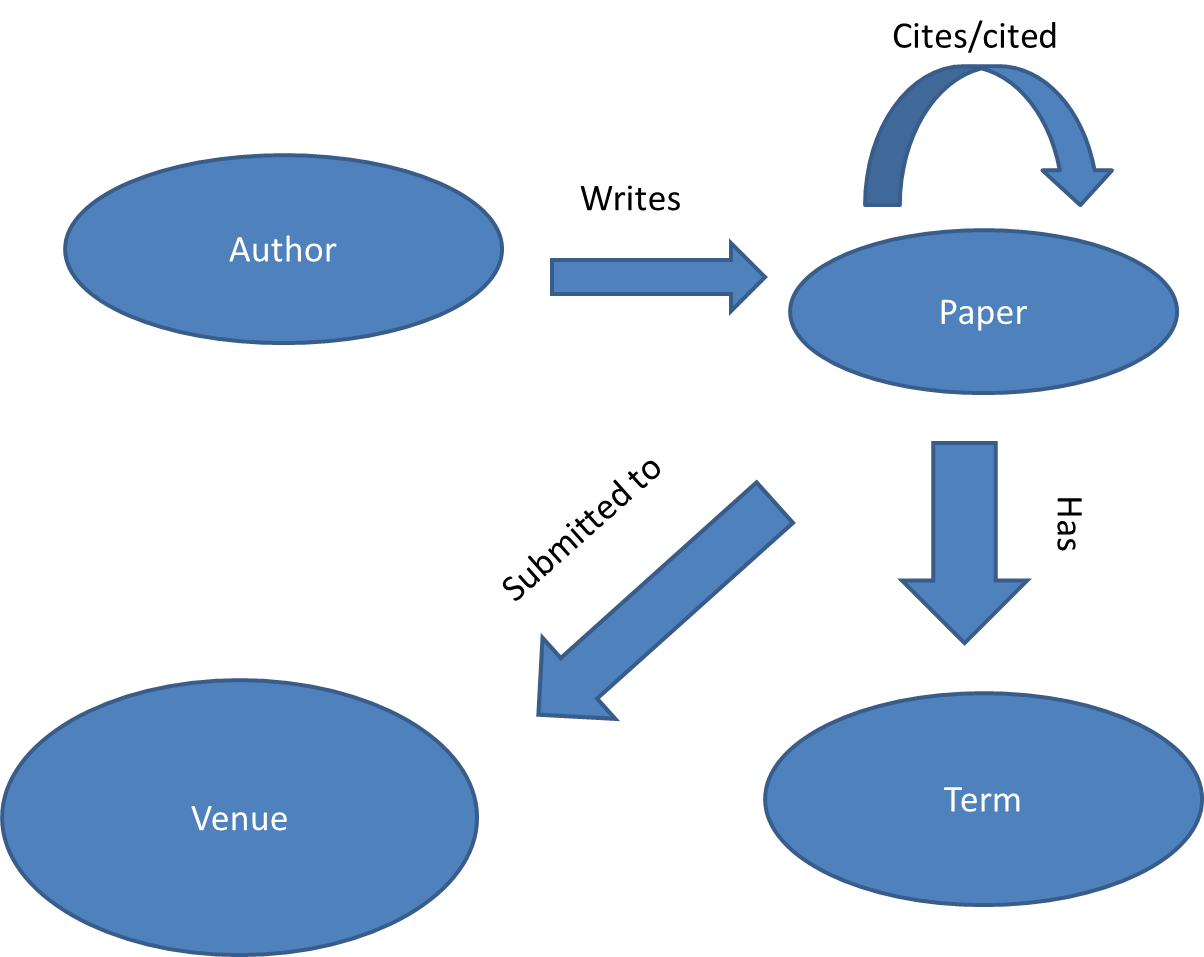
\includegraphics[width=0.6\linewidth]{./figs/relationship.png}
    \caption{Bibliographic Network}
    \label{fig:relationship}
\end{figure}

PathSim strives to define similarity measures between objects in heterogeneous
information network using structural information and to answer top-k similarity
search queries efficiently. It accomplishes this by developing a novel meta
path-based framework.

As shown in Figure~\ref{fig:relationship}, entities can be connected via
different connectivity paths. For instance, two authors can be connected via
author-paper-author (i.e. co-authors) path or author-paper-venue-paper-author
(i.e.  the authors submitted both of their papers to the same conferences)
path. Intuitively, the different paths represent a different similarity
semantics. More formally, as written in the paper, the meta-path can be
described as follows:

\begin{Def}
\label{meta-path}
\textbf{Meta path}. A meta path $\mathcal{P}$ is a path defined on the graph on
network schema $\mathcal{T_G} = \mathcal{(A, R)}$, and is denoted in the form
of $\mathcal{A}_1 \xrightarrow{R_1} \mathcal{A}_2 \xrightarrow{R_2} \cdots
\xrightarrow{R_l} \mathcal{A}_{l + 1}$ which defines a composite relation
$\mathcal{R} = \mathcal{R}_1 \circ \mathcal{R}_2 \circ \cdots \circ
\mathcal{R}_l$ where $\circ$ denotes the composition operator on relations. \newline
\end{Def}

Although multiple similarities measure have been previously explored such as
path counting or random walk-based similarity, they are biased to either
popular entities and thus unable to capture the essence of peer similarity.
For instance, if we would like to find out about authors that are similar to
an early PhD student that has published a few papers, the above measures
will yield professors who happen to co-author with this particular student
although what we desire are other PhD students. This has become the other
motivation for PathSim. Using the concept of meta-path above, Path-Sim
defines the relationship between two entities as follow: \newline

\begin{Def}
\label{path-sim}
\textbf{PathSim: A Meta path-based similarity measure}. Given a symmetric
meta path $\mathcal{P}$, PathSim between two objects of the same type
x and y is:

\begin{align*}
s(x,y)=\frac{2*|\{p_{x \rightsquigarrow x}:p_{x \rightsquigarrow y}\}|\in\mathcal{P}}
{|\{p_{x \rightsquigarrow x}:p_{x \rightsquigarrow x}\}|\in\mathcal{P} +
|\{p_{y \rightsquigarrow y}:p_{y \rightsquigarrow y}\}|\in\mathcal{P}}
\end{align*}

where $p_{a \rightsquigarrow b}$ is the meta-paths between $a$ and $b$. \newline
\end{Def}

Intuitively, this indicates that if $x$ is popular, but not $y$, the number of
meta-paths between $x$ and itself will be much larger than the number of
meta-paths between $x$ and $y$. Thus, when we are comparing a popular entity
and an un-popular entity $s(x,y)$ will be low and vice versa. We need to have
either both to be popular or un-popular so that $s(x,y)$ yield a considerable
value.

\subsection{hPathSim}

There are three main improvements that we made to the PathSim framework.

\subsection{Hierarchy Forest}

The heterogeneous network contains hierarchies for certain entities. For example,
a location hierarchy could look like:

\begin{align*}
Urbana \leadsto USA \leadsto North America \leadsto root
\end{align*}

\h builds a forest of hierarchical trees, the trees are using HashTables in their core to 
allow for fast lookup of a node in the tree. The roll-up and drill-down operations
on the tree are implemented just by using a depth-first search (DFS).

The forest provides 5 key operations for each of the trees:
\begin{itemize}
    \item \textit{is\_member(nodeTitle, queryID)}: Applies an iterative DFS to check if 
    the node with id \textit{queryID} is under the subtree of \textit{nodeTitle}.
    \item \textit{is\_slice(nodeTitle, queryID)}: check whether the node with $nodeTitle$
    has the id $queryID$.
    \item \textit{get\_categories()}: return the tree titles in the forest.
    \item \textit{get\_children(nodeTitle)}: get all immediate children under the node 
    $nodeTitle$.
    \item \textit{get\_parent(nodeTitle)}: get the parent of the node $nodeTitle$.
\end{itemize}

All the operations described above take $O(1)$ run-time due to the HashTable, except for 
\textit{is\_member} which can take $O(N)$ where $N$ is the number of nodes under the specified 
hierarchy tree.
